\documentclass[a4paper]{article}

\usepackage[francais]{babel}
\usepackage{xltxtra,fontspec,xunicode}

\usepackage{listings}

\usepackage{graphicx}
\usepackage{float}

\begin{document}
\section{Introduction}
Le but de ce project et de réaliser un application de tracking GPS, qui 
permet à un ensemble d'utilisateur de partager leur trajets en temps réel.

\begin{figure}[H]
  \begin{center}
  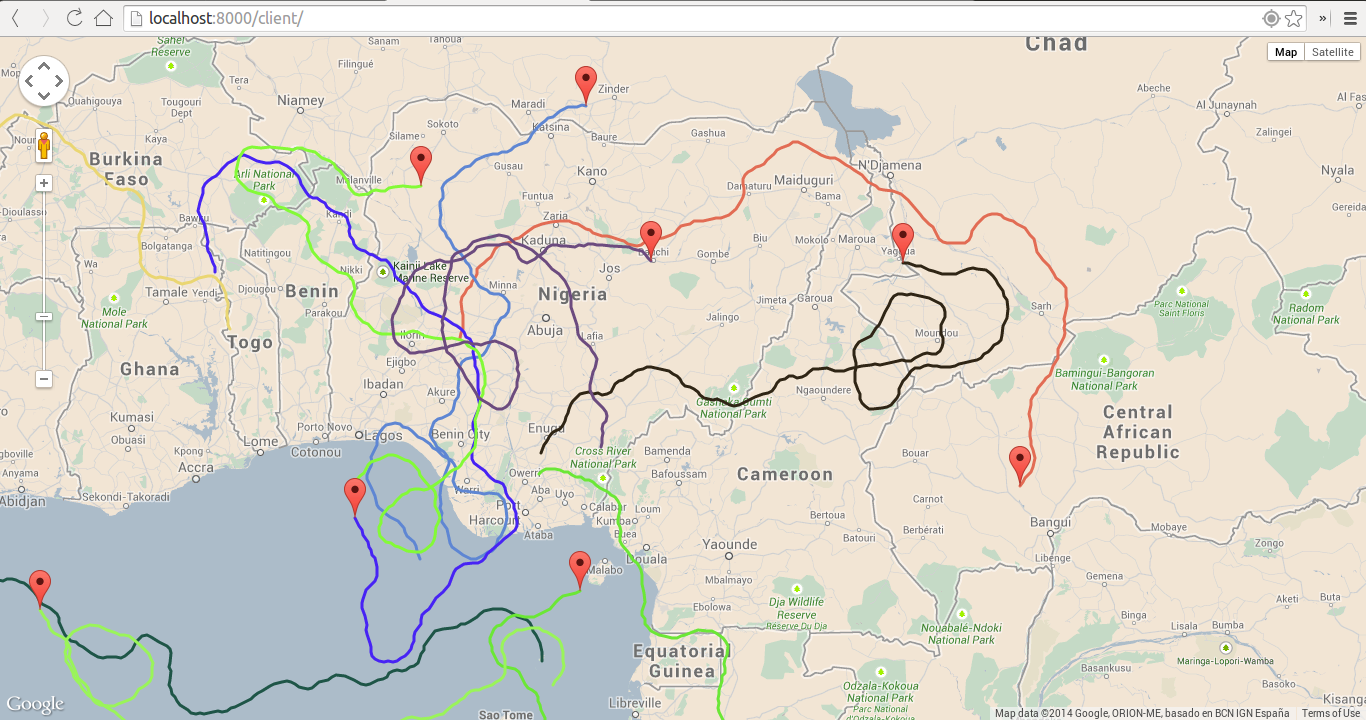
\includegraphics[scale=0.25]{screenshot.png}
  \end{center}
\end{figure}

Afin de réliser cette application nous avons utiliser les outils suivant :

\section{Outils utilisés}
\subsection{Node.js}

\begin{figure}[H]
  \begin{center}
  
\includegraphics[scale=0.5]{nodejs.png}
  \end{center}
\end{figure}

Node.js est une plateforme logicielle libre et événementielle en 
JavaScript orientée vers les applications réseau.

Elle utilise la machine virtuelle V8 et implémente sous 
licence MIT les spécifications CommonJS. 

Node.js contient une bibliothèque de 
serveur HTTP intégrée, ce qui rend possible de faire tourner un serveur 
web sans avoir besoin d'un logiciel externe comme Apache ou Lighttpd, 
et permettant de mieux contrôler la façon dont le serveur web fonctionne.

\subsection{Socket.io}

\begin{figure}[H]
  \begin{center}
  
\includegraphics[scale=1]{socketio.png}
  \end{center}
\end{figure}

Socket.io est un framework pour les application temps-réel. Il est composé de deux 
partie une partie client qui tourne sur un navigateur et une autre serveur qui tourne sur Node.js.
Le deux parties ont une API identique.

La technologie principale que Socket.io est le protocol WebSockets, mais il
peut utiliser d'autre méthodes comme Flash, Long-polling, JSONP.

\subsection{Angular.js}

\begin{figure}[H]
  \begin{center}
  
\includegraphics[scale=1]{angularjs.png}
  \end{center}
\end{figure}

Angular.js est un framework Javascript coté client dévélopé par Google
qui à pour but d'accélerer le développement d'application web monopages.
Il propose d'étendre la syntax de HTML avec des balise personnlisé, organiser 
l'application sous une architecture MVC, communiquer avec le serveur, routing, 
data-binding et autres fonctionnalités.

\subsection{Phantom.js et Casper.js}

\begin{figure}[H]
  \begin{center}
  
\includegraphics[scale=0.5]{phantomjs.png}
  
\includegraphics[scale=0.2]{casperjs.png}
  \end{center}
\end{figure}

Phantom.js et un headless browser c'est un dire une navigateur qui sans interface
graphique mais plutot une API qui permet d'écrire des tests pour les applications
web coté client.

Casper.js est framework de Phantom.js qui facilite l'écriture de ces scripts.

\section{Réalisation}

\subsection{Serveur}

Le code suivant utilise le framework express pour servir les fichier html, css et Javascript
qui se trouve dans le dossier client
et lance le serveur HTTP sur le port `port' : 

\begin{lstlisting}
var express = require('express')
  , http = require('http');

// create http server
var app = express()
  , server = http.Server(app);

// serve client's static files
app.use('/client', express.static(__dirname + '/../client'));

// run the server
var port = process.argv[2] || 8000;
server.listen(port, function() {
  console.log('Server started : http://localhost:' + port + '/client');
});
\end{lstlisting}



\end{document}

